\section{Theorie}
\label{sec:Theorie}

% In knapper Form sind die physikalischen Grundlagen des Versuches, des Messverfahrens, sowie sämtliche für die Auswertung erforderlichen Gleichungen darzustellen. (Keine Herleitung)

% (eventuell die Aufgaben)

% Der Versuchsaufbau: Beschreibung des Versuchs und der Funktionsweise (mit Skizze/Bild/Foto)

Wenn ein System durch eine Änderung der Umgebungsbedingungen aus seinem Anfangszustand entfernt wird und daraufhin nicht-oszillatorisch in diesen zurückkehrt, kann man Relaxationseffekte beobachten. \autoref{fig:schaltung_1} ist eine Schaltung dargestellt, mit der diese Relaxationsphänomene beobachten werden können , das Auf- und Entladen eines Kondensators über einen Widerstand. 
Befindet sich der Schalter in \autoref{fig:schaltung_1} in Stellung eins, so entlädt sich der Kondensator mit der Kapazität $C$. Auf seinen beiden Platten liegt die Ladung Gesamtladung $Q$. Dadurch liegt zwischen den beiden Kondensatorplatten eine Spannung von 

\begin{figure}
    \centering
    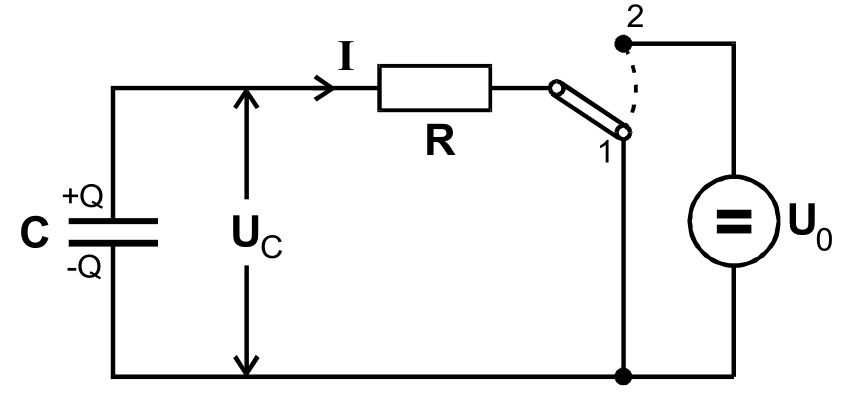
\includegraphics[width=\textwidth/2]{images/schaltung_1.png}
    \caption{Schaltbild eines RC-Kreises, der in Stellung 1 entladen und in Stellung 2 geladen wird. \cite{V353}}
    \label{fig:schaltung_1}
\end{figure}

\begin{equation}
    \label{eq:kondensatorspannung}
    U_C = \frac{Q}{C}.
\end{equation}

Durch das ohmsche Gesetz ist bekannt, dass durch diese Spannung $U_C$ und den Widerstand $R$ ein Strom 

\begin{equation}
    \label{eq:ohmschesgesetz}
    I = \frac{U_C}{R}
\end{equation}

verursacht wird. 
Der zeitliche Verlauf der Ladung $Q$ auf dem Kondensator $C$, beim Entladen, kann durch eine Exponentialfunktion beschrieben werden, dadurch ergibt sich

\begin{equation}
    \label{eq:entladungsladung}
    Q (t) = Q (0) \exp{\left(\frac{-t}{RC} \right)}.
\end{equation}

Wobei $RC$ eine Zeitkonstante ist, die im nächsten Abschnitt näher erklärt wird. \cite{V353}
Äquivalent dazu lässt sich der Aufladevorgang eines Kondensators $C$ durch die Spannung $U_0$ über den Widerstand $R$ beschreiben. Hierbei gelten folgende Randbedingungen für $Q$

\begin{align}
    \label{eq:ladung}
    Q (0) = 0 && Q (\infty) = C \cdot U_0.
\end{align}

Damit lässt sich der Aufladevorgang durch

\begin{equation}
    \label{eq:aufladungsladung}
    Q (t) = C \cdot U_0  (1- \exp{\left(\frac{-t}{RC} \right)} )
\end{equation}

beschreiben. \cite{V353} Dabei ist $RC$ wieder die Zeitkonstante aus \autoref{eq:entladungsladung}, mit dieser Konstante kann beschrieben werden, wie schnell sich ein System seinem Endzustand annähert. Die Zeitkonstante wird druch die Kapazität $C$ und den Widerstand $R$ im RC-Kreis festgelegt. Nachdem eine Zeit von 
\begin{equation}
    \Delta T = RC
\end{equation} verstrichen ist, ändert sich die Kondensatorladung $Q$ um den Faktor
\begin{equation}
    \label{eq:RC1}
    \frac{Q (t = RC)}{Q (0)} = \frac{1}{e} \approx 0.386.
\end{equation}

Um den Wert $RC$ aus experimentellen Daten zu bestimmen, wenn $R$ und $C$ unbekannt sind wird \autoref{eq:RC1} in eine andere Form gebracht. In der neuen Form

\begin{equation}
    \label{eq:RC2}
    \ln \left( \frac{Q (t)}{Q (0)} \right) = t \cdot \frac{-1}{RC}
\end{equation}

kann man $RC$ als negative reziproke Steigung einer halblogarithmischen Funktion sehen.\cite{V353}

Eine periodische Auslenkung aus der Gleichgewichtslage erzeugt ebenfalls Relaxationsphänomene und kann ebenfalls mit einem RC-Kreis untersucht werden. 

\begin{figure}
    \centering
    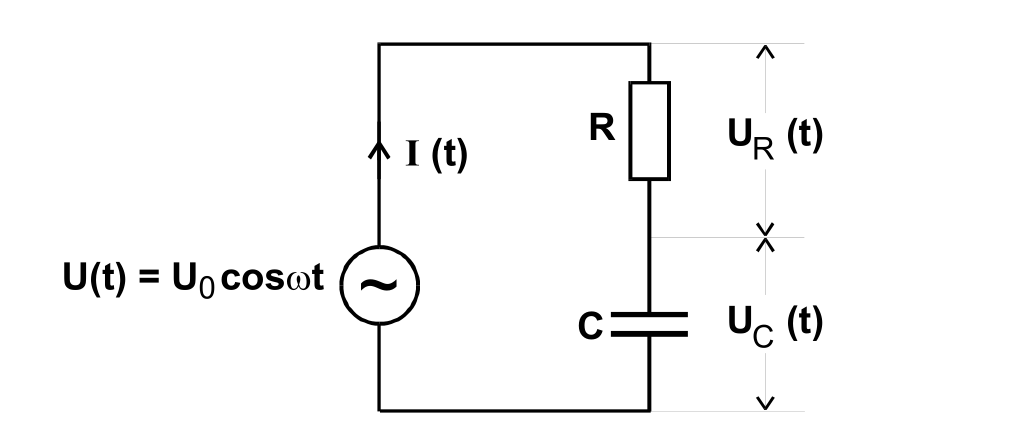
\includegraphics[width=\textwidth/2]{images/schaltung_2.png}
    \caption{Mögliches Schaltbild zur Entstehung eines Relaxationsphänomens durch periodische Anregung.  \cite{V353}}
    \label{fig:schaltung_2}
\end{figure}

Wird die Schaltung aus \autoref{fig:schaltung_2} durch die Wechselspannung $U (t)$ mit der Kreisfrequenz $\omega$ angetrieben, also 

\begin{equation}
    \label{eq:wechselspannung}
    U (t) = U_0 \cdot \cos \left(\omega t \right),
\end{equation}

so ändert sich das Verhalten des RC-Kreises in Anhängigkeit von der Frequenz. Für $\omega \ll \frac{1}{RC}$ werden die Kondensatorspannung $U_C$ und die Generatorspannung $U (t)$ in \autoref{eq:wechselspannung} etwa gleich sein, da der Kondensator genug Zeit hat sich vollständig aufzuladen, bevor die Spannung wieder abfällt und ihr Vorzeichen ändert. Bei entsprechend höheren Frequenzen kann der Aufladevorgang nicht mehr vollständig stattfinden und die Amplitude $A$ der Kondensatorspannung wird kleiner werden. Sie ist gegeben durch

\begin{equation}
    \label{eq:amplitude}
    A (\omega) = \frac{U_0}{\sqrt{1 + \omega^2 R^2 C^2}}.
\end{equation}

Durch die verzögerte Aufladung entsteht eine Phasenverschiebung $\varphi$, die sich bei ansteigender Frequenz asymptotisch dem Wert $\varphi = \frac{\pi}{2}$ annähert. Wie an

\begin{equation}
    \label{eq:phasenverschiebung}
    \varphi (\omega) = \arctan \left(-\omega R C \right)
\end{equation}

auch zu erkennen ist. Alternativ lässt sich die Phasenverschiebung auch über die zeitlichen Verläufe von $U_C$ und $U_0$ berechnen, dafür müssen die Schwingungsdauer $T$ bzw. $b$ in \autoref{fig:phasenmessung} und der zeitliche Abstand der Nulldurchgänge $a$ bekannt sein. Die Schwingungsdauer $b$ ist die Inverse der eingestellten Frequenz $f$.

\begin{figure}
    \centering
    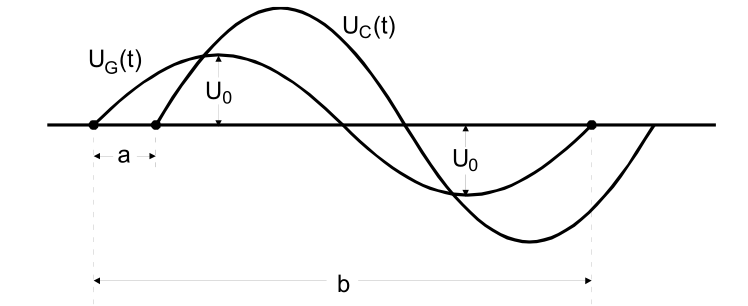
\includegraphics[width=\textwidth/2]{images/phasenmessung.png}
    \caption{Darstellung der Methode zur Berechnung der Phasenverschiebung  \cite{V353}}
    \label{fig:phasenmessung}
\end{figure}

\autoref{fig:phasenmessung} stellt das Prinzip genauer da. Über den Zusammenhang

\begin{equation}
    \label{eq:phasenverschiebung2}
    \varphi = a \cdot f \cdot 2\pi = \frac{a}{T} \cdot 2\pi
\end{equation}

lässt sich die Phasenverschiebung berechnen.
Außerdem lässt sich aus \autoref{eq:amplitude} und \autoref{eq:phasenverschiebung} der Zusammenhang
\begin{equation}
    \label{eq:spannung_phase}
    \frac{A(\varphi)}{U_0} = \cos(\varphi)
\end{equation}
zeigen, welcher die Spannungsamplitude in Abhängigkeit der Phasenverschiebung aufzeigt.

Aus der Eigenschaft, nur niedrige Frequenzen passiern zu lassen, kann \autoref{fig:schaltung_2} als ein Tiefpass verwendet werden. \cite{V353}
Die Schaltung aus \autoref{fig:schaltung_2} besitzt noch eine weitere Eigenschaft, sie kann als ein sogenannter Integrator verwendet werden. Für $\omega \gg \frac{1}{RC}$ gilt die Beziehung

\begin{align}
    \label{eq:integrator}
    U (t) = RC \: \frac{\mathrm{d} U_C}{\mathrm{d}t}  && U_C (t) = \frac{1}{RC} \int _0^t U (t') \mathrm{d} t'.
\end{align}

Dadurch wird zu der Generatorspannung $U (t)$ eine Kondensatorspannung $U_C (t)$ erzeugt, die sich nur durch einen Faktor von der Stammfunktion von $U(t)$ unterscheidet. \cite{V353}